%%%%%%%%%%%%%%%%%%%%
%%%%%%%%%%%%%%%%%%%%
%%
%% Andrea Tino - 2019
%% Programming + Science
%% Opinion model
%%
%%%%%%%%%%%%%%%%%%%%
%%%%%%%%%%%%%%%%%%%%

\section{Building our first CA: Conway's Game of Life}
\label{sec:simpleca}

We want to create our first CA in code, so that we can display the cells and see them changing
state. In this section, we will build the basic architecture of a CA that can be used to build any
CA in future. For this, we are going to use the latest web technologies to create web sites and
web applications in the browser: Javascript, HTML and CSS.

\subsection{Creating the basic project structure}
In our PC, let's create a directory (anywhere you want, on your Desktop maybe?) and give it
a cool name like: \texttt{cellautom}. Inside this new directory, do the following:

\begin{enumerate}
\item Create a file and name it: \texttt{index.html}.
\item Create a file and name it: \texttt{ca.js}.
\item Create one last file and name it: \texttt{style.css}.
\end{enumerate}

These three files represent the basic organization of our visual CA we are going to develop.
Table \ref{tab:files} offers a good overview of what they are needed for.

%
% Table
%
\begin{table}[!t]
\centering
\caption{List of files in our project folder.}
\label{tab:files}
%
% Follow this input for your own table layout
%
\begin{tabular}{p{0.2\textwidth}p{0.2\textwidth}p{0.5\textwidth}}
\hline\noalign{\smallskip}
File & Type & Description \\
\noalign{\smallskip}\svhline\noalign{\smallskip}
\texttt{index.html} & Web page & This is the web page that will display the CA and its evolution.\\
\texttt{ca.js} & Javascript code file  & This file will contain the Javascript
code that will make the CA appear and evolve.\\
\texttt{style.css} & CSS Stylesheet & The stylesheet we will use to apply colors, fonts 
    and make our CA beautiful.\\
\noalign{\smallskip}\hline\noalign{\smallskip}
\end{tabular}
\end{table}
%

% Figure
%
\begin{figure}[b]
\sidecaption
% tikz diagram
\input{diag-dirstruct1}
%
% If not, use
%\picplace{5cm}{2cm} % Give the correct figure height and width in cm
%
\caption{Your project folder should look like this.}
\label{fig:dirstruct1}
\end{figure}
%

\subsection{Defining the barebones}
Time to write the initial code to see something appear on the page once we run it in the browser.
Open file \texttt{index.html} with your favorite editor.

\begin{programcode}{index.html}
Write this code minding casing and spacing.
\begin{codehtml}
<!DOCTYPE html>
<html>
<head>
  <title>My Cellular Automaton</title>
</head>

<body>
  Hello world!
</body>
</html>
\end{codehtml}
\end{programcode}

Save the file and now try to open it in your browser: we have just displayed a text!

\begin{tips}{Learning point - A first glance at HTML}
The code we just wrote is read by the browser to create a graphical visualization. HTML is used to
create web pages. It is not a \textit{programming language} (it does not tell a computer what to do),
but a \textit{markup language} (it tells a computer what to display and paint on the screen).

A minimal HTML page looks exactly like the one we just wrote.
It is all based on the concept of \textit{tags}. The
first line \texttt{<!DOCTYPE html>} is special and tells the browser that we are using the latest
version of HTML (you should always use this). Then a new tag \texttt{<html>} is opened and is
closed at the end of the file: \texttt{</html>}. An opening tag and a closing tag make a \textit{block}.
Blocks can contain other blocks.

The \texttt{<html>} block must contain, in order, two other blocks:
\texttt{<head>} and \texttt{<body>}. The first block contains the \texttt{<title>}
block for defining the title of the page
(this text is displayed on the browser's top bar). Everything inside \texttt{<head>} will not generate any 
graphics, it only contains information about the page. What's inside \texttt{body} is, on the other hand, 
painted (or, more technically speaking, rendered\footnote{The term \textit{render} is used to indicate
the complex set of operations that a program does in order to visualize something on the screen.})
inside the browser window. As you can see, we only have a piece of 
text\footnote{The \textit{Hello World} is, historically, the first thing one learns
to do when studying and playing with a new language, we had to respect tradition here.}, which
is in fact rendered on a blank, empty page.
\end{tips}

Of course, we don't just want to display text, we want to render a full CA! So, in the same file, replace
that text.

\begin{programcode}{index.html (snippet)}
Remove \texttt{Hello world!} and insert a \texttt{<div>} block instead.
\begin{codehtmlh1}{1}{3}
<body>
  <div id="ca"></div>
</body>
\end{codehtmlh1}
\end{programcode}

A \texttt{<div>} block is used to group things. We are going to write some code that puts some graphics
inside it. Before leaving this file, we need to import inside it the other two files we have created.

\begin{programcode}{index.html (snippet)}
Place these new tags right below block \texttt{<title>}.
\begin{codehtmlh1}{2}{5}
<head>
  <title>My Cellular Automaton</title>
  <script src="ca.js"></script>
  <link rel="stylesheet" href="style.css">
</head>
\end{codehtmlh1}
\end{programcode}

The first new tag we have added is a \texttt{<script>} which instructs the browser to load and run the
Javascript code inside \texttt{ca.js}. The next one is a \texttt{<link>} tag (this one does not have a closing
tag\footnote{Some tags do not have a closing tag and some do. There is not a rule, you just have
to memorize.})
and tells the browser to load the styles defined inside \texttt{style.css}. As of now, if you refresh the
page in the browser, you will just see a blank page (not for long!).

\subsection{Creating the grid}
For now, we are done with \texttt{index.html}; the next step is to write the code to render the automaton
in our page. To do this, let's open \texttt{ca.js} and insert the first lines of code.

\begin{programcode}{ca.js}
These first lines of Javascript code create our \textit{module}.
\begin{code}
(function(){
  // This is a module
})();
\end{code}
\end{programcode}

We have just created a \textit{module}, let's try to understand a bit more about them.

\begin{tips}{Learning point - Javascript modules}
Javascript language does not have an intrinsic concept of module, this is something programmers create in
different ways. A \textit{module} is a programming structure encapsulating some code that is isolated
from other codes running in the page.

It is a very generic definition because there is really not much more about it. For now, everytime
we write some code that needs to run in the page, we will wrap it inside a module like shown before,
this is a standard procedure to make sure other Javascript codes on the page, in future, do not
affect our code. Modules also guarantee that our code does not have any side
effects on other scripts running on the same page.
\end{tips}

We have imported \texttt{ca.js} inside \texttt{index.html}, so when we refresh the page the module
we wrote will run. However, since there is really no code inside the module (just a comment),
nothing will happen. Our objective here is to render a grid of cells which will be our automaton,
to achieve this, let's start by defining a few constants:

\begin{programcode}{ca.js}
Define the constants we will use at the beginning on the module.
\begin{codeh1}{1}{5}
(function(){
  const rowsnum = 9;
  const colsnum = 9;
  const cellsize = 20; // In px
})();
\end{codeh1}
\end{programcode}

The constants we defined will be used to create an automaton of the size we specify in 
\texttt{rowsnum} and \texttt{colsnum}. Constant \texttt{cellsize} will be used to defined the
width and height of each (square) cell. Moving on, we now want to create the code that renders the grid.

\begin{programcode}{ca.js}
Inside the module, after the constants, add a function and the code to invoke it.
\begin{codeh1}{5}{13}
(function(){
  const rowsnum = 9;
  const colsnum = 9;
  const cellsize = 20; // In px

  function create() {
    // Here the code to create the grid
  }

  window.addEventListener("load", function() {
    create();
  });
})();
\end{codeh1}
\end{programcode}

We have added two things: we have defined function \texttt{create}, and we have added some code in
the module that uses \texttt{window.addEventListener}. This is what happens when we run the page:

\begin{enumerate}
\item The module is executed.
\item Function \texttt{window.addEventListener} is run. This code will register a function (the one
passed as second parameter) and invoke it, once the event specified in the first parameter fires.
\item When the page has finished loading and everything is ready, function \texttt{create} is called.
\end{enumerate}

If we didn't use \texttt{window.addEventListener}, but just executed \texttt{create()}, our
application might fail sometimes. This code guarantees that we start doing things only when
the page is fully loaded; we need this guard and it is good practice to always write it.

\begin{programcode}{ca.js (snippet)}
Add a new function after function \texttt{create} inside the module.
\begin{codeh1}{4}{8}
function create() {
  // Here the code to create the grid
}

function getContainer() {
  return document.getElementById("ca");
}
\end{codeh1}
\end{programcode}

Function \texttt{getContainer} is going to be important for us later. This function simply
uses \texttt{document.getElementById} to retrieve the \texttt{<div>} we added before in
\texttt{index.html} (we do this by using the \texttt{id} property on the tag).
At this point, we are ready to fill function
\texttt{create} with the code which renders the grid inside the page.

\begin{programcode}{ca.js (snippet)}
Focusing on function \texttt{create}, remove the comment and add this code instead.
\begin{codeh1}{1}{16}
function create() {
  let container = getContainer();
  container.style.width = (colsnum * cellsize + colsnum) + "px";

  for (let i = 1; i <= rowsnum; i++) {
    for (let j = 1; j <= colsnum; j++) {
      let cell = document.createElement("div");
      cell.id = i + ":" + j;
      cell.classList.add("cell");
      cell.style.width = cellsize + "px";
      cell.style.height = cellsize + "px";

      container.appendChild(cell);
    }
  }
}
\end{codeh1}
\end{programcode}

% Figure
%
\begin{figure}[b]
\sidecaption
% tikz diagram
%
% Tikz Diagram
%

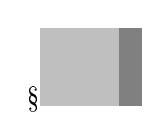
\begin{tikzpicture}

\tikzmath{
	\S = 0.7;
}

\fill[lightgray] (0,0) rectangle (1,1);
\fill[gray] (1,0) rectangle (1.3,1);

\end{tikzpicture}

%
% If not, use
%\picplace{5cm}{2cm} % Give the correct figure height and width in cm
%
\caption{The drawing strategy for the grid
is simple: we decide to add a padding between the container
and its content of \texttt{1px} (from the top and from the left);
the same amount is used to set a right and bottom margin in each cell. Using this spacing
technique, we separate the cells from the container and the cells from each other by the same
amount. The background of the container is set to black, and the one of each cell to white, so
that, in the end, the final effect is that of a grid with white cells and black borders.}
\label{fig:gridlayout}
\end{figure}
%

The code above does a few things. In the first lines, we get a reference to the CA container
(the \texttt{<div>} in the page), and set its width according to the size we specified in the
constants. Later on, we create a row-by-column scanning by using one loop nested into the other.
The outer loop will be used to set the current row, the inner loop to set the column. The code
inside the two loops will be executed $\text{rowsnum} \times \text{colsnum}$ times
(for each cell to create).

The code inside the loops first creates a \texttt{<div>} block, then assigns it an id (very
important step, so that we can reference each cell later
by using \texttt{document.getElementById}), adds a style class to it and defines its width and height.
The last command invokes \texttt{appendChild} on the container: this will make the cell appear
inside the container.\\

Try to refresh the page! What can you see? Not really what we were hoping right? Well, the fact that
we cannot see much does not mean that the page is empty. Let's have a look by inspecting the page
using the F12 tool. If we do so, the tool will display, under the \textit{Elements} tab, the
content of the page: our \texttt{<div>}s are there, it's just that the browser is not rendering
them on the page the way we want. The problem is styling, we must properly style the elements we
have created by using some CSS.

\begin{programcode}{style.css}
Insert this code in \texttt{style.css}.
\begin{codecss}
body {
  margin: 10px;
  padding: 10px;
}

#ca {
  background-color: #000;
  display: flex;
  flex-wrap: wrap;
  padding-left: 1px;
  padding-top: 1px;
}

.cell {
  border: none;
  background-color: #fff;
  margin-right: 1px;
  margin-bottom: 1px;
  flex: 0 0 auto;
}
\end{codecss}
\end{programcode}

We have filled the stylesheet with 3 sets of rules. The first set is for the \texttt{<body>} element
and just defines a 10 pixel spacing between the borders and the content of the whole page.
The second targets
the container (as it has \texttt{id="ca"}): we set the background to black and
make sure all contained cells wrap by using \texttt{display: flex} and \texttt{flex-wrap: wrap}.
Figure \ref{fig:gridlayout} will help you understand how we get the final result by using the
style we just wrote.

% Figure
%
\begin{figure}[b]
\sidecaption
% tikz diagram
%
% Tikz Diagram
%

\begin{tikzpicture}

\tikzmath{
	\W = 3;
	\H = 2;
	\n = 5;
	\s = \W / \n;
	\i = 0.2; % Inter-margin
	\d = 1; % Displacement between the two
	\Bix1 = 0;
	\Bfx1 = \Bix1 + \W;
	\Biy1 = 0;
	\Bfy1 = \Biy1 + \H;
	\six1 = \Bix1 + \i;
	\siy1 = \Bfy1 - \i;
	\sfx1 = \six1 + \s;
	\sfy1 = \siy1 - \s;
	\six2 = \sfx1 + \i;
	\siy2 = \H - \i;
	\sfx2 = \six2 + \s;
	\sfy2 = \siy1 - \s;
	\six3 = \sfx2 + \i;
	\siy3 = \H - \i;
	\sfx3 = \six3 + \s;
	\sfy3 = \siy1 - \s;
	\six4 = \sfx3 + \i;
	\siy4 = \H - \i;
	\sfx4 = \six4 + \s;
	\sfy4 = \siy1 - \s;
	\six5 = \sfx4 + \i;
	\siy5 = \H - \i;
	\sfx5 = \six5 + \s;
	\sfy5 = \siy1 - \s;
	\Bix2 = \Bix1 - \W - \d;
	\Bfx2 = \Bix2 + \W;
	\Biy2 = 0;
	\Bfy2 = \Biy2 + \H;
	\six6 = \Bix2 + \i;
	\siy6 = \Bfy2 - \i;
	\sfx6 = \six6 + \s;
	\sfy6 = \siy6 - \s;
	\six7 = \sfx6 + \i;
	\siy7 = \Bfy2 - \i;
	\sfx7 = \six7 + \s;
	\sfy7 = \siy6 - \s;
	\six8 = \sfx7 + \i;
	\siy8 = \Bfy2 - \i;
	\sfx8 = \six8 + \s;
	\sfy8 = \siy6 - \s;
	\six9 = \six6;
	\siy9 = \sfy6 - \i;
	\sfx9 = \sfx6;
	\sfy9 = \siy9 - \s;
	\six0 = \six7;
	\siy0 = \sfy6 - \i;
	\sfx0 = \sfx7;
	\sfy0 = \siy9 - \s;
	\Ax = \sfx8;
	\Ay = \siy8 + (\sfy8 - \siy8) * 0.5;
	\Bx = \Ax + \i;
	\By = \Ay - \i;
	\Dx = \six9;
	\Dy = \siy9 + (\sfy9 - \siy9) * 0.5;
	\Cx = \Dx - \i;
	\Cy = \Dy + \i;
	\tx1 = (\Bfx1 - \Bix1) * 0.5;
	\ty1 = \Biy1 - 0.2;
	\tx2 = (\Bfx2 - \Bix2) * 0.5 + \Bix2;
	\ty2 = \ty1;
}

\filldraw[fill=white, draw=black] (\Bix1,\Biy1) rectangle (\Bfx1,\Bfy1);
\filldraw[fill=lightgray, draw=gray] (\six1,\siy1) rectangle (\sfx1,\sfy1) node[pos=.5] {\tiny \texttt{.cell}};
\filldraw[fill=lightgray, draw=gray] (\six2,\siy2) rectangle (\sfx2,\sfy2) node[pos=.5] {\tiny \texttt{.cell}};
\filldraw[fill=lightgray, draw=gray] (\six3,\siy3) rectangle (\sfx3,\sfy3) node[pos=.5] {\tiny \texttt{.cell}};
\filldraw[fill=lightgray, draw=gray] (\six4,\siy4) rectangle (\sfx4,\sfy4) node[pos=.5] {\tiny \texttt{.cell}};
\filldraw[fill=lightgray, draw=gray] (\six5,\siy5) rectangle (\sfx5,\sfy5) node[pos=.5] {\tiny \texttt{.cell}};

\filldraw[fill=white, draw=black] (\Bix2,\Biy2) rectangle (\Bfx2,\Bfy2);
\filldraw[fill=lightgray, draw=gray] (\six6,\siy6) rectangle (\sfx6,\sfy6) node[pos=.5] {\tiny \texttt{.cell}};
\filldraw[fill=lightgray, draw=gray] (\six7,\siy7) rectangle (\sfx7,\sfy7) node[pos=.5] {\tiny \texttt{.cell}};
\filldraw[fill=lightgray, draw=gray] (\six8,\siy8) rectangle (\sfx8,\sfy8) node[pos=.5] {\tiny \texttt{.cell}};
\filldraw[fill=lightgray, draw=gray] (\six9,\siy9) rectangle (\sfx9,\sfy9) node[pos=.5] {\tiny \texttt{.cell}};
\filldraw[fill=lightgray, draw=gray] (\six0,\siy0) rectangle (\sfx0,\sfy0) node[pos=.5] {\tiny \texttt{.cell}};

\draw[thick,->,red] plot [smooth] coordinates {(\Ax,\Ay) (\Bx,\By) (\Cx,\Cy) (\Dx,\Dy)};

\node[] at (\tx1,\ty1) {\texttt{<div id="\#ca">}};
\node[] at (\tx2,\ty2) {\texttt{<div id="\#ca">}};

\end{tikzpicture}

%
% If not, use
%\picplace{5cm}{2cm} % Give the correct figure height and width in cm
%
\caption{Flex wrapping explained. The right-most diagram shows a container without wrapping,
while the left-most shows the same situation where the container is set to wrap its children.}
\label{fig:flexwrap}
\end{figure}
%

\begin{tips}{Learning point - CSS Flex wrap}
CSS has many features and allows styling HTML elements in many different ways. One of the coolest tricks
is \textit{flex-wrapping}. Wrapping (in general) means that
when a bunch of elements are lined up in a row and they reach the
end of their container, instead of shrinking or overflowing, they automatically go down below to start a
new row as shown in figure \ref{fig:flexwrap}. This is the most common case: \textit{horizontal wrapping},
however, there is also \textit{vertical wrapping} where elements form columns.

To enable wrapping we need to work on two different sets of elements: one container element, and many
contained elements (they must be direct children of the container). The container must be styled to
be a \textit{flex-container}, and we achieve this by setting \texttt{display: flex}. Another property
must be set on the container: \texttt{flex-wrap: wrap}, this will make the flex-container a
\textit{wrapping container}, so that all its direct children would wrap when reaching the borders of it.
Once that's accomplished, we must make sure children do not change in size when filling the container.
In flex containers, CSS tries to fit everything where it can; so, if we leave things as they are, we might
not get the desired result: we must tell the browser not to change the size of the contained elements, so that
they wrap; we achieve this by setting \texttt{flex: 0 0 auto} on the contained children.
\end{tips}

If you try to refresh the page now, you will see the grid!

\begin{trailer}{Media content}
You can find the code for this project up to this point in folder \texttt{v2.3}.
\end{trailer}

\begin{problem}
\label{prob:changecasize}
Change the size of the CA/grid by setting it to different dimensions. Also try to make rectangular
automata, not just square grids.
\end{problem}

\subsection{Coding the evolution logic}
We have succeeded rendering the grid, but at the moment our CA doesn't do much, it does nothing!
The key feature of CA is, as we learned at the beginning of this chapter, their ability to
\textit{evolve}. We need to write down that
logic\footnote{Developers use the term \textit{logic} a lot to refer to a behavior that they need
to develop for an application. In our case, we need to code the behavior of evolution in the CA,
so that it can change configuration during every cycle. You can replace the word
\textit{behavior} with \textit{logic}, as many among software engineers and programmers like to
use the latter in their everyday jargon.}.

But what kind of CA are we going to build? What is the state going to be? How about the neighborhood? We
need to define all these properties. The CA we are going to build is a simple and very famour one called:
\textit{Conway's Game of Life} (CGL) \cite{wolfram-ca}.
This CA has the following characteristics:

\begin{itemize}
\item The set of states (alphabet) is: $\mathcal{A} = \{ 0, 1 \}$, where $0$ means "off" (inactive, dead) and
$1$ means "on" (active, alive).
\item Each cell has a Moore neighborhood (recall definition \ref{def:neighmoore} and example \ref{ex:simpleca}).
\item The CA describes pixels in a screen. When a pixel (cell) is on, it turns black; when it's off, it
turns white. 
\end{itemize}

This CA was the first ever published in the history of Mathematics, and it has very interesting properties.

\subsubsection{Setting the initial state}
In CA, it is crucial that we are able to set the initial condition (remember what we talked about in
theorem \ref{theo:evinitcond}). To do so, let's add this code.

\begin{programcode}{ca.js (snippet)}
Insert this constant in \texttt{ca.js} right after the existing contants at the beginning of the module.
\begin{codeh1}{1}{3}
const cellsize = 20; // In px
const initConfig = ["2:2", "4:7", "7:4", "5:5", "3:8"];
\end{codeh1}
\end{programcode}

The line we have added defines a constant which will hold the array of cell identifiers with an initial state
of $1$ in the CA. The code we have at the moment simply creates the cells and nothing more;
as soon as we finish rendering the grid, we must set the initial state.

\begin{programcode}{ca.js (snippet)}
Add this function just below function \texttt{create} inside the module.
\begin{code}
function initializeGrid() {
  for (let i = 1; i <= rowsnum; i++) {
    for (let j = 1; j <= colsnum; j++) {
      if (initConfig.indexOf(i + ":" + j) >= 0) {
        set(i, j, 1);
      } else {
        set(i, j, 0);
      }
    }
  }
}
\end{code}
\end{programcode}

We are going to invoke \texttt{initializeGrid} right after the grid is rendered. As you can see, we traverse
all cells by scanning them row by column as we did before. Inside both loops, we invoke function \texttt{set}
(this function does not exist yet, we will write it in a moment) which will configure the cell state to either
$0$ or $1$ depending on whether the cell identifier is in the \texttt{initConfig} list or not. This will allow us
to set the initial configuration of the CA.

\begin{important}{Bottom-up vs. top-down programming}
We cannot execute the code at this time yet because we still need to write function \texttt{set}.
This approach we have chosen now is a bit different from before. Previously, if, say, function $B$ had to
be called inside function $A$, we would write function $B$ first, and then write down function $A$. Now we are
doing the opposite. The first approach is called \textit{bottom-up programming}
as we build from the foundations and then add on top.
The latter is called \textit{top-down programming} because we start from the higher levels, then moving down
writing what's needed.

The good thing of bottom-up coding is that it's possible to gradually test and run the code at 
every step, but the final algorithm takes
shape later. On the other end, top-down programming is cumbersome, because we cannot test our progress until
all the layers have been built, but the code takes the final shape from the very beginning.
\end{important}

We have written the function responsible for initializing the CA, but we have only defined it, no place in code
is invoking it. We need to invoke it, where? As we mentioned, this phase must occur right after the grid is
rendered; who renders the grid? That would be function \texttt{create}, and who calls that function? If you
scroll down in \texttt{ca.js}, you see that, at the end of the module, the module itself calls it!

\begin{programcode}{ca.js (snippet)}
Invoke function \texttt{initializeGrid} right after calling \texttt{create}.
\begin{codeh1}{2}{4}
window.addEventListener("load", function(){
  create();
  initializeGrid();
});
\end{codeh1}
\end{programcode}

At this point we have almost everything, as soon as the page starts, the grid is created and then
\texttt{initializeGrid} will be called to set the initial state. However that function is trying to
call \texttt{set}, which is another function we still need to define. The purpose of function
\texttt{set(row, column, value)} will be to set the value of the cell at position
$(\text{row}, \text{column})$ to the value in parameter \texttt{value}: $0$ means off and $1$ means on.

\begin{programcode}{ca.js (snippet)}
Add this function right below \texttt{initializeGrid}.
\begin{code}
function set(i, j, value) {
  let cell = getCell(i, j);
  cell.setAttribute("data-value", value);
}
\end{code}
\end{programcode}

The function will first try to get the HTML element of the cell, and then it will try to set attribute
\texttt{data-value} to that. As you can see, here as well we are doing top-down programming because
function \texttt{getCell} does not yet exist, we need to write it.

\begin{programcode}{ca.js (snippet)}
Add this function right above \texttt{set}.
\begin{code}
function getCell(i, j) {
  return document.getElementById(i + ":" + j);
}
\end{code}
\end{programcode}

When we created the grid, we set an identifier to every cell element. Function \texttt{document.getElementById}
is present in every browser and it returns the first HTML element whose \texttt{id} corresponds to the one
provided as input. At this point it seems like everything is done, so try and refresh the page; unfortunately
you will not see anything different. Did we make any mistake? Let's try to see.

\begin{enumerate}
\item Open the browser and refresh the page. You should see the grid.
\item Open the F12 tools and navigate to the \textit{Elements} panel.
\item Expand the \texttt{<body>} tag. Also expand the \texttt{<div id="ca" ...>} tag.
\end{enumerate}

You should, at this point, see the list of \texttt{<div>} tags that represent the cells. See how, in correspondance
of the IDs in array \texttt{initConfig}, the tag shows \texttt{data-value="1"} (\texttt{data-value="0"}
otherwise). So our logic is actually working. The actual problem is the styling. We want the cells marked with
\texttt{data-value="1"} to appear as black, and not white. So let's head to \texttt{style.css} and make some
modifications.

\begin{programcode}{style.css (snippet)}
Add this code at the bottom of the file.
\begin{codecss}
.cell[data-value="1"] {
  background-color: #000;
}
\end{codecss}
\end{programcode}

Make sure you always save. The code we just added instructs the browser to apply a black background color
to our cells when their HTML elements have attribute \texttt{data-value} set to \texttt{1}.
Now our code is finished and we can refresh the page to see our CA getting an initial
condition.

\begin{problem}
\label{prob:changeinit}
Change the initial condition of the grid. Set to \textit{on} only the following
cells: $(3,1)$, $(1,3)$ and $(4,4)$.
\end{problem}

\subsubsection{Building the UI}
At this point we have succeeded setting the initial condition. This means that we can configure the CA however
we want by just changing array \texttt{initConfig} at the beginning of the module. Our final goal is to
make the CA evolve and see it as it changes. We need to build a \textit{User Interface} (or simply: \textit{UI})
that gives us the ability to:

\begin{enumerate}
\item Render the CA in its next configurartion. We can accomplish this with a button: every time we
click this button, the CA will shift to its next configuration from the current one.
\item Visualize what iteration we are in. We can create a piece of text that displays a number
representing the index of the current configuration (discrete time).
\end{enumerate}

So we basically need to create 2
\textit{controls}\footnote{A web page, or more generally, a user interface in every application or app, is made
of different things: buttons, texts, text boxes, input fields and so on. Each one of them is a piece of the UI,
one common way to refer to them is by using the word: \textit{control} in design jargon.}: one button and
one text label. We want to display them at the bottom of the grid, on the left.

\begin{programcode}{index.html (snippet)}
Add a new \texttt{<div>} block right after the one containing the CA.
\begin{codehtmlh1}{2}{5}
<body>
  <div id="ca"></div>
  <div class="controls">
  </div>
</body>
\end{codehtmlh1}
\end{programcode}

The new \texttt{<div>} we just added will be the container for our button and text label. Next step
is adding them inside their container.

\begin{programcode}{index.html (snippet)}
Place these new lines inside the \texttt{<div>} block we added a moment ago.
\begin{codehtmlh1}{1}{4}
<div class="controls">
  <button id="buttonNext">Next</button>
  <span id="cycleText"></span>
</div>
\end{codehtmlh1}
\end{programcode}

Tag \texttt{<button>} creates, as you probably already figured out, a button. While tag \texttt{<span>}
is used to show text. If you go ahead and refresh the page, you will see the button, but no
label next to it. That is because we need to put some text inside it. Since the text in the label
must show the current CA's iteration, we need to track time.

\begin{programcode}{ca.js (snippet)}
Create a variable in the module right after constant \texttt{initConfig} (add spaces before and after to
have a nice code formatting by separating constants, variables and functions in the module).
\begin{codeh1}{3}{5}
const cellsize = 20; // In px
const initConfig = ["3:4", "3:5", "4:3", "4:4", "5:4"];

let t = 0; // Cycles (time)

function create() {
\end{codeh1}
\end{programcode}

Variable \texttt{t} will keep track of time by storing the current CA's iteration. As you can see, when the
module starts, its initial value is set to \texttt{0}, because the initial configuration is cycle 0!
Now we need to show the value of \texttt{t} in the label we just created. To do this, we create a function
which will update the label text:

\begin{programcode}{ca.js (snippet)}
Add this function in the last part of the module.
\begin{codeh1}{0}{5}
function updateCycleText() {
  let text = document.getElementById("cycleText");
  text.textContent = "cycle " + t;
}

window.addEventListener("load", function () {
\end{codeh1}
\end{programcode}

As you can see, function \texttt{updateCycleText} will first locate the label in our page by using
\texttt{document.getElementById} and ID \texttt{"cycleText"} we placed on that element; so that later
we can access the element's \texttt{textContent} and set it to the value we want. We will invoke
this function everytime the CA moves to the next configuration but also when the CA is first created.
This last part we can actually do now.

\begin{programcode}{ca.js (snippet)}
Invoke function \texttt{updateCycleText} right after we call the function to initialize the grid in
the last part of the module.
\begin{codeh1}{3}{5}
window.addEventListener("load", function () {
  create();
  initializeGrid();
  updateCycleText();
});
\end{codeh1}
\end{programcode}

If we refresh the page now, we will see the label next to the button showing text: "cycle 0". Of course,
if we press the button, nothing happens because we haven't written anything for that yet, so let's add
the code to react and do something when the button is clicked.

\begin{programcode}{ca.js (snippet)}
Add this function in the module right after function \texttt{initializeGrid}.
\begin{code}
function initializeButton() {
  let button = document.getElementById("buttonNext");
  button.addEventListener("click", function(){
    console.log("You have clicked me!");
  });
}
\end{code}
\end{programcode}

This function will search for the button element in the page and then add a listener for the \texttt{click}
event. It means that the function we pass as second parameter to \texttt{addEventListener} will be executed
every time the button is clicked. At the  moment we will just display a message in the console. We
of course need to call function \texttt{initializeButton} to make this happen, we invoke the function
right after the grid has been initialized.

\begin{programcode}{ca.js (snippet)}
Invoke function \texttt{initializeButton} right after we call the function to initialize the grid in
the last part of the module.
\begin{codeh1}{3}{5}
window.addEventListener("load", function () {
  create();
  initializeGrid();
  initializeButton();
  updateCycleText();
});
\end{codeh1}
\end{programcode}

If you refresh the page, make sure the F12 tools are open and visible on your screen, and click the button:
you will see the message appearing in the console.

\subsubsection{Coding the evolution}
Everything is prepared now. We have the CA initialized and we also have the UI to interact with the CA.
Next step is creating the logic to make the automaton evolve.
This piece of code will be executed when we press the button.

\begin{programcode}{ca.js (snippet)}
In function \texttt{initializeButton}, remove the line of code to print to console, and write these lines
instead.
\begin{codeh1}{3}{6}
function initializeButton() {
  let button = document.getElementById("buttonNext");
  button.addEventListener("click", function(){
    next();
    updateCycleText();
  });
}
\end{codeh1}
\end{programcode}

Every time we click the button we do 2 things:

\begin{enumerate}
\item We first move the CA to the next configuration by using
function \texttt{next} (which does not exist yet, we will write it later).
\item We invoke function \texttt{updateCycleText} to update the time label.
\end{enumerate}

Let's write down function \texttt{next} which is the core of the evolution logic we need to develop.

\begin{programcode}{ca.js (snippet)}
Add these lines after function \texttt{set}.
\begin{code}
function next() {
  // Calculate the values
  // Todo

  // Apply the values
  // Todo

  t++;
}
\end{code}
\end{programcode}

We haven't really written the whole logic. Since function \texttt{next} will need to do a few things, we
have just prepared it by defining the 3 main actions. As you can see, we have basically created 3 phases:

\begin{enumerate}
\item Calculating the new states for each cell.
\item Applying the states.
\item Incrementing (updating) time.
\end{enumerate}

% Figure
%
\begin{figure}[b]
\sidecaption
% tikz diagram
%
% Tikz Diagram
%

\begin{tikzpicture}

\tikzmath{
	\S = 0.7cm;
  \May1 = 0;
  \Mby1 = -4;
}

\tikzset{square matrix/.style={
    matrix of nodes,
    column sep=-\pgflinewidth, row sep=-\pgflinewidth,
    nodes={draw,
      minimum height=#1,
      anchor=center,
      text width=#1,
      align=center,
      inner sep=0pt
    },
  },
  square matrix/.default=\S
}

\matrix[square matrix] (m1) at (0,\May1)
{
\phantom{} & \phantom{} & \phantom{} & \phantom{} \\
\phantom{} &|[preaction={fill, lightgray}, pattern=north west lines, pattern color=black]| \phantom{} & \phantom{} & \phantom{} \\
\phantom{} & \phantom{} & \phantom{} & \phantom{} \\
};
\draw[opacity=.5, ultra thick, red] (m1-1-1.north west)-|
   (m1-3-3.south east)-|
   (m1-3-1.south west)-|cycle;
\draw [->, thick] (m1-2-2.center) -- (m1-1-1.center);
\draw [->, thick] (m1-2-2.center) -- (m1-1-2.center);
\draw [->, thick] (m1-2-2.center) -- (m1-1-3.center);
\draw [->, thick] (m1-2-2.center) -- (m1-2-1.center);
\draw [->, thick] (m1-2-2.center) -- (m1-2-3.center);
\draw [->, thick] (m1-2-2.center) -- (m1-3-1.center);
\draw [->, thick] (m1-2-2.center) -- (m1-3-2.center);
\draw [->, thick] (m1-2-2.center) -- (m1-3-3.center);

\matrix[square matrix] (m2) at (0,\Mby1)
{
\phantom{} & \phantom{} & \phantom{} & \phantom{} \\
\phantom{} &|[preaction={fill, lightgray}, pattern=north west lines, pattern color=black]| \phantom{} &|[preaction={fill, lightgray}, pattern=north west lines, pattern color=black]| \phantom{} & \phantom{} \\
\phantom{} & \phantom{} & \phantom{} & \phantom{} \\
};
\draw[opacity=.5, ultra thick, red] (m2-1-2.north west)-|
   (m2-3-4.south east)-|
   (m2-3-2.south west)-|cycle;
\draw [->, thick] (m2-2-3.center) -- (m2-1-2.center);
\draw [->, thick] (m2-2-3.center) -- (m2-1-3.center);
\draw [->, thick] (m2-2-3.center) -- (m2-1-4.center);
\draw [->, thick] (m2-2-3.center) -- (m2-2-2.center);
\draw [->, thick] (m2-2-3.center) -- (m2-2-4.center);
\draw [->, thick] (m2-2-3.center) -- (m2-3-2.center);
\draw [->, thick] (m2-2-3.center) -- (m2-3-3.center);
\draw [->, thick] (m2-2-3.center) -- (m2-3-4.center);

\node[text width=2cm] at (2.85,0) {$t = k$};
\node[text width=2cm] at (2.85,-4) {$t = k+1$};

\draw [->, double] (0,-1.5) -- (0,-2.5);

\end{tikzpicture}

%
% If not, use
%\picplace{5cm}{2cm} % Give the correct figure height and width in cm
%
\caption{An example of incremental CA. As you can see in iteration $t=k$, one cell is updated
with its new state. In the next iteration ($t=k+1$), the next cell is updated, however its state
will be calculated on the new value of the previous.}
\label{fig:updatecainc}
\end{figure}
%

% Figure
%
\begin{figure}[b]
\sidecaption
% tikz diagram
%
% Tikz Diagram
%

\begin{tikzpicture}

\tikzmath{
	\S = 0.7cm;
  \D = 5.5;
  \d = 1.6;
  \MAx = 0.5;
  \MBx = \MAx;
  \Maax = 0;
  \Mbbx = \Maax;
  \MAy = -1.6;
  \MBy = \MAy - \D;
  \Maay = \MAy + \d;
  \Mbby = \MBy + \d;
}

\tikzset{square matrix/.style={
    matrix of nodes,
    column sep=-\pgflinewidth, row sep=-\pgflinewidth,
    nodes={draw,
      minimum height=#1,
      anchor=center,
      text width=#1,
      align=center,
      inner sep=0pt
    },
  },
  square matrix/.default=\S
}

\matrix[square matrix] (mg1) at (\MAx,\MAy)
{
\phantom{} & \phantom{} & \phantom{} & \phantom{} \\
\phantom{} &|[preaction={fill, lightgray}, pattern=north west lines, pattern color=black]| \phantom{} & \phantom{} & \phantom{} \\
\phantom{} & \phantom{} & \phantom{} & \phantom{} \\
};
\matrix[square matrix] (m1) at (\Maax,\Maay)
{
|[fill=white]| \phantom{} &|[fill=white]| \phantom{} &|[fill=white]| \phantom{} &|[fill=white]| \phantom{} \\
|[fill=white]| \phantom{} &|[fill=white]| \phantom{} &|[fill=white]| \phantom{} &|[fill=white]| \phantom{} \\
|[fill=white]| \phantom{} &|[fill=white]| \phantom{} &|[fill=white]| \phantom{} &|[fill=white]| \phantom{} \\
};
\draw[opacity=.5, ultra thick, red] (m1-1-1.north west)-|
   (m1-3-3.south east)-|
   (m1-3-1.south west)-|cycle;
\draw [->, thick] (m1-2-2.center) -- (m1-1-1.center);
\draw [->, thick] (m1-2-2.center) -- (m1-1-2.center);
\draw [->, thick] (m1-2-2.center) -- (m1-1-3.center);
\draw [->, thick] (m1-2-2.center) -- (m1-2-1.center);
\draw [->, thick] (m1-2-2.center) -- (m1-2-3.center);
\draw [->, thick] (m1-2-2.center) -- (m1-3-1.center);
\draw [->, thick] (m1-2-2.center) -- (m1-3-2.center);
\draw [->, thick] (m1-2-2.center) -- (m1-3-3.center);

\matrix[square matrix] (mg2) at (\MBx,\MBy)
{
\phantom{} & \phantom{} & \phantom{} & \phantom{} \\
\phantom{} &|[preaction={fill, lightgray}, pattern=north west lines, pattern color=black]| \phantom{} &|[preaction={fill, lightgray}, pattern=north west lines, pattern color=black]| \phantom{} & \phantom{} \\
\phantom{} & \phantom{} & \phantom{} & \phantom{} \\
};
\matrix[square matrix] (m2) at (\Mbbx,\Mbby)
{
|[fill=white]| \phantom{} &|[fill=white]| \phantom{} &|[fill=white]| \phantom{} &|[fill=white]| \phantom{} \\
|[fill=white]| \phantom{} &|[fill=white]| \phantom{} &|[fill=white]| \phantom{} &|[fill=white]| \phantom{} \\
|[fill=white]| \phantom{} &|[fill=white]| \phantom{} &|[fill=white]| \phantom{} &|[fill=white]| \phantom{} \\
};
\draw[opacity=.5, ultra thick, red] (m2-1-2.north west)-|
   (m2-3-4.south east)-|
   (m2-3-2.south west)-|cycle;
\draw [->, thick] (m2-2-3.center) -- (m2-1-2.center);
\draw [->, thick] (m2-2-3.center) -- (m2-1-3.center);
\draw [->, thick] (m2-2-3.center) -- (m2-1-4.center);
\draw [->, thick] (m2-2-3.center) -- (m2-2-2.center);
\draw [->, thick] (m2-2-3.center) -- (m2-2-4.center);
\draw [->, thick] (m2-2-3.center) -- (m2-3-2.center);
\draw [->, thick] (m2-2-3.center) -- (m2-3-3.center);
\draw [->, thick] (m2-2-3.center) -- (m2-3-4.center);

\node[text width=2cm] at (2.75,0) {$t = k$};
\node[text width=2cm] at (2.75,-5.5) {$t = k+1$};

\draw [->, double] (0,-3) -- (0,-4);

\end{tikzpicture}

%
% If not, use
%\picplace{5cm}{2cm} % Give the correct figure height and width in cm
%
\caption{An example of immediate CA. By using a temporary CA (a ghost CA) we can update
the state of the cells of the CA without polluting our calculations. After all cells have been scanned, the
ghost CA is used to replace the saved states in the original CA. At the end of the process, the ghost CA is
finally destroyed as no more needed.}
\label{fig:updatecaimm}
\end{figure}
%

We are going to replace the \texttt{// Todo} comments with actual code, but now we need to explain a few
things about why we have decided to use this approach, why we have defined these 2 phases: 
\textit{calculate} and \textit{apply}. Our strategy is to:

\begin{enumerate}
\item Scan all the cells in the CA (as we did before) and calculate the state for each cell.
The new states will be memorized in a temporary location.
\item In the second phase, we are going to scan again the cells, and we will apply the new states.
\end{enumerate}

Why do we want to scan the cells twice? Can't we just scan the cells one time and apply each new state
right after calculating it? The answer is no, because otherwise we would calculate the CA's new configuration
in an undesired way. Look at figure \ref{fig:updatecainc},
the diagram shows what happens if we do not use the double
scanning and the problem of polluting the grid. For this reason we need to scan the cells twice. This is because
our CA is going to be an \textit{immediate CA}, it means that all the cells update at the same time
as shown in figure \ref{fig:updatecaimm}.
With the other
approach, we would otherwise have an \textit{incremental CA}, where every new configuration of a cell depends on the
newly updated value of the neighbors. Incremental CA are not wrong automata,
they are just different. In this chapter,
however, we want to use immediate CA!

In an immediate CA, the states of all cells can actually be updated in parallel. But we are not going to go
that far here (the code for doing this is much more complicated).

We need to talk about one last thing before resuming coding: the \textit{border effect}. We know how to
calculate the next configuration of a CA: we need to compute all the new states of all the cells. And the state
of a cell depends on the state of its neighbors. Normally a cell has 8 neighbors as we explained in definition
\ref{def:neigh}, however the cells on the border have fewer neighbors as shown in figure \ref{fig:bordercells}:

\begin{itemize}
\item If a cell is on the border, it will have 3 neighbors less, for a total of 5.
\item A corner cell loses 5 neighbors, for a total of 3.
\end{itemize}

% Figure
%
\begin{figure}[b]
\sidecaption
% tikz diagram
%
% Tikz Diagram
%

\begin{tikzpicture}

\tikzmath{
  \S = 0.4cm;
  \X1 = 0;
  \X2 = -3;
  \X3 = -6;
  \Y1 = 0;
  \Yf = \Y1 - 1.3;
}

\tikzset{square matrix/.style={
    matrix of nodes,
    column sep=-\pgflinewidth, row sep=-\pgflinewidth,
    nodes={draw,
      minimum height=#1,
      anchor=center,
      text width=#1,
      align=center,
      inner sep=0pt
    },
  },
  square matrix/.default=\S
}

\matrix[square matrix] (m1) at (\X1,\Y1)
{
\phantom{} & \phantom{} & \phantom{} & \phantom{} & \phantom{} \\
\phantom{} &|[fill=lightgray]| \phantom{} &|[fill=lightgray]| \phantom{} &|[fill=lightgray]| \phantom{} & \phantom{} \\
\phantom{} &|[fill=lightgray]| \phantom{} &|[fill=black]| \phantom{} &|[fill=lightgray]| \phantom{} & \phantom{} \\
\phantom{} &|[fill=lightgray]| \phantom{} &|[fill=lightgray]| \phantom{} &|[fill=lightgray]| \phantom{} & \phantom{} \\
\phantom{} & \phantom{} & \phantom{} & \phantom{} & \phantom{} \\
};
\draw[opacity=.5, ultra thick, red] (m1-2-2.north west)-|
   (m1-4-4.south east)-|
   (m1-4-2.south west)-|cycle;
\node[] at (\X1,\Yf) {(normal)};

\matrix[square matrix] (m2) at (\X2,\Y1)
{
\phantom{} & \phantom{} & \phantom{} & \phantom{} & \phantom{} \\
|[fill=lightgray]| \phantom{} &|[fill=lightgray]| \phantom{} & \phantom{} & \phantom{} & \phantom{} \\
|[fill=black]| \phantom{} &|[fill=lightgray]| \phantom{} & \phantom{} & \phantom{} & \phantom{} \\
|[fill=lightgray]| \phantom{} &|[fill=lightgray]| \phantom{} & \phantom{} & \phantom{} & \phantom{} \\
\phantom{} & \phantom{} & \phantom{} & \phantom{} & \phantom{} \\
};
\draw[opacity=.5, ultra thick, red] (m2-2-1.north west)-|
   (m2-4-2.south east)-|
   (m2-4-1.south west)-|cycle;
\node[] at (\X2,\Yf) {(border)};

\matrix[square matrix] (m3) at (\X3,\Y1)
{
|[fill=black]| \phantom{} &|[fill=lightgray]| \phantom{} & \phantom{} & \phantom{} & \phantom{} \\
|[fill=lightgray]| \phantom{} &|[fill=lightgray]| \phantom{} & \phantom{} & \phantom{} & \phantom{} \\
\phantom{} & \phantom{} & \phantom{} & \phantom{} & \phantom{} \\
\phantom{} & \phantom{} & \phantom{} & \phantom{} & \phantom{} \\
\phantom{} & \phantom{} & \phantom{} & \phantom{} & \phantom{} \\
};
\draw[opacity=.5, ultra thick, red] (m3-1-1.north west)-|
   (m3-2-2.south east)-|
   (m3-2-1.south west)-|cycle;
\node[] at (\X3,\Yf) {(corner)};

\end{tikzpicture}

%
% If not, use
%\picplace{5cm}{2cm} % Give the correct figure height and width in cm
%
\caption{A visualization of the neighborhoods of border and corner cells.
It is clearly possible to see how, when compared to a normal cell, border cells have 5 neighbors and
corner cells have 3 instead of 8.}
\label{fig:bordercells}
\end{figure}
%

What do we do with them? There are many approaches: we could have special rules for them when updating their
state for instance.

\begin{example}[Using different rules for border and corner cells]
\label{ex:diffruleset}
Consider a CA where every cell can either be active or inactive, like the LED CA in
example \ref{ex:stateled}; in this automaton we set a transition rule for which 
a cell becomes active only if at least half of its neighbors are active. For a
normal cell that number is 4, but for a border cell or corner cell? We could use a special rule for border
cells and set that number to 2 or 3, and for corner cells we could set that number to 1 or 2.
\end{example}

Using different rules for cells (as suggested in example \ref{ex:diffruleset})
makes the automaton more complex though, and we don't want that.
So we are going to
choose the simplest approach: ignoring border and corner cells. It means that, when computing the next
configuration of a CA, we are not going to update the state of border and corner cells, they will always retain their initial state. Practically speaking, it means that our scanning will exclude border and corner cells
(we will see this in action in code soon). With all this in mind, let's go back to code.

\begin{programcode}{ca.js (snippet)}
Replace the \texttt{// Todo} comments with the following lines.
\begin{codeh2}{2}{8}{9}{15}
function next() {
  // Calculate the values
  for (let i = 2; i <= rowsnum - 1; i++) {
    for (let j = 2; j <= colsnum - 1; j++) {
      // This is the first scan
    }
  }

  // Apply the values
  for (let i = 2; i <= rowsnum - 1; i++) {
    for (let j = 2; j <= colsnum - 1; j++) {
      // This is the second scan
    }
  }

  t++;
}
\end{codeh2}
\end{programcode}

The scanning blocks here are different from those we wrote inside function \texttt{create}.
Look at the indices in the \texttt{for} loops: this time they start from
$2$ not $1$. And they finish with $rowsnum - 1$ and $colsnum - 1$ instead of $rowsnum$ and $colsnum$.
When we do this, we are effectively excluding from the scan all border and corner cells.

We are now ready to start calculating the next state of every cell, however we don't know what
transition rule to follow.

\begin{definition}[State transition rules in Conway's Game of Life]
\label{def:cglrules}
In CGL CA, the transition rules are the following:
\begin{enumerate}
\item Any \textbf{active} cell with fewer than 2 active neighbors becomes \textbf{inactive}.
\item Any \textbf{active} cell with 2 or 3 active neighbors remains \textbf{active}.
\item Any \textbf{active} cell with more than 3 active neighbors becomes \textbf{inactive}.
\item Any \textbf{inactive} cell with exactly 3 active neighbors becomes \textbf{active}.
\item If none of the above rules apply, the cell's state remains \textbf{the same}.
\end{enumerate}
\end{definition}

The first thing we wanna do is translating the rules in definition \ref{def:cglrules} into
actual Javascript code inside our module.

\begin{programcode}{ca.js (snippet)}
Add this code in the module right below function \texttt{next}.
\begin{code}
function calculateState(state, neighSum) {
  if (state === 1 && neighSum < 2) {
    return 0; // Any active cell with fewer than 2 active neighbors becomes inactive
  }
  if (state === 1 && neighSum >= 2 && neighSum <= 3) {
    return 1; // Any active cell with 2 or 3 active neighbors remains active
  }
  if (state === 1 && neighSum > 3) {
    return 0; // Any active cell with more than 3 active neighbors becomes inactive
  }
  if (state === 0 && neighSum === 3) {
    return 1; // Any inactive cell with exactly 3 active neighbors becomes active
  }
  return state; // Otherwise the cell's state remains the same
}
\end{code}
\end{programcode}

Function \texttt{calculateState} implements the 5 rules in the CA as per definition \ref{def:cglrules} and
can be used to calculate the next state of a single cell.
It accepts 2 arguments: \texttt{state} is the cell's current state, and \texttt{neighSum} is the number of
neighbor cells that are active in the current configuration (cycle).
We are going to use this function inside \texttt{next}.

\begin{programcode}{ca.js (snippet)}
Remove comment \texttt{// This is the first scan} from the first scanning double loop and add this
code instead.
\begin{codeh1}{2}{16}
for (let i = 2; i <= rowsnum - 1; i++) {
  for (let j = 2; j <= colsnum - 1; j++) {
    // Cell (i,j)'s state
    let cell = get(i, j);

    // States of cell (i,j)'s neighbors
    let north = get(i - 1, j);
    let south = get(i + 1, j);
    let east = get(i, j + 1);
    let west = get(i, j - 1);
    let northeast = get(i - 1, j + 1);
    let southeast = get(i + 1, j + 1);
    let northwest = get(i - 1, j - 1);
    let southwest = get(i + 1, j - 1);
    let sum = north + south + east + west + northeast + southeast + northwest + southwest;
  }
}
\end{codeh1}
\end{programcode}

% Figure
%
\begin{figure}[b]
\sidecaption
% tikz diagram
%
% Andrea Tino
% 2020
%
% =======================================================================
% Creative Commons Attribution-NonCommercial-ShareAlike 4.0 International
% Public License
% =======================================================================
%

\begin{tikzpicture}

\tikzmath{
	\S = 0.7cm;
}

\tikzset{square matrix/.style={
    matrix of nodes,
    column sep=-\pgflinewidth, row sep=-\pgflinewidth,
    nodes={draw,
      minimum height=#1,
      anchor=center,
      text width=#1,
      align=center,
      inner sep=0pt
    },
  },
  square matrix/.default=\S
}

\matrix[square matrix] (m1) at (0,0)
{
$\dots$ & $\dots$ & $\dots$ & $\dots$ & $\dots$ \\
$\dots$ & |[fill=lightgray]| $y_{\begin{subarray}{l}i-1\\j-1\end{subarray}}$ &|[fill=lightgray]| $y_{\begin{subarray}{l}i-1\\j\end{subarray}}$ &|[fill=lightgray]| $y_{\begin{subarray}{l}i-1\\j+1\end{subarray}}$ & $\dots$ \\
$\dots$ & |[fill=lightgray]| $y_{\begin{subarray}{l}i\\j-1\end{subarray}}$ &|[fill=black,text=white]| $y_{i,j}$ &|[fill=lightgray]| $y_{\begin{subarray}{l}i\\j+1\end{subarray}}$ & $\dots$ \\
$\dots$ & |[fill=lightgray]| $y_{\begin{subarray}{l}i+1\\j-1\end{subarray}}$ &|[fill=lightgray]| $y_{\begin{subarray}{l}i+1\\j\end{subarray}}$ &|[fill=lightgray]| $y_{\begin{subarray}{l}i+1\\j+1\end{subarray}}$ & $\dots$ \\
$\dots$ & $\dots$ & $\dots$ & $\dots$ & $\dots$ \\
};

\end{tikzpicture}

%
% If not, use
%\picplace{5cm}{2cm} % Give the correct figure height and width in cm
%
\caption{A visualization of the neighborhood of a cell in the grid.
A generic cell $(i,j)$ is highlighted in the CA (black)
and its neighborhood is visualized (in grey).
Note how the coordinates of each neighbor cell is expressed relatively
to cell $(i,j)$.}
\label{fig:cellneigh}
\end{figure}
%

The code we have added is needed to collect all the info we need to calculate the next state for every cell.
Recall that in a CA, the new state of a cell is calculated by using:

\begin{itemize}
\item The cell's current state.
\item The current states of the cell's neighbors.
\end{itemize}

We are using top-down programming again by invoking function \texttt{get} (which does not exist yet). This function
will return a cell's current state by passing its row and column number. Apart from that, the code we
just wrote is not dificult to understand: we first get the state of the cell we are scanning, then we get the states
of its neighbors. Figure \ref{fig:cellneigh} provides a good visualization to better understand the code we just
wrote.
We compute 9 variables in total and then we create variable \texttt{sum} which will
contain the number of active neighbors (remember that an active cell has state $1$, $0$ otherwise). In this
code, there is one more thing left to do: calculating the new state and saving it.

\begin{programcode}{ca.js (snippet)}
Always inside the first double loop, add these lines at the end.
\begin{codeh1}{2}{5}
let sum = north + south + east + west + northeast + southeast + northwest + southwest;

// Calculate new state and save it
setTmp(i, j, calculateState(cell, sum));
\end{codeh1}
\end{programcode}

Function \texttt{setTmp} (which we still need to write, yes more top-down programming) will save the new state
for the currently scanned cell in the ghost CA (without polluting the original automaton).
The first two parameters are the row and the column of the cell whose
new state we need to save, the third parameter is the value of the new state, of course we use function
\texttt{calculateState} (which we wrote before) for this task. We have used top-down programming quite often here,
let's write down the code of what's missing: we need to define two functions: \texttt{get} and \texttt{setTmp}.

\begin{programcode}{ca.js (snippet)}
In the module, add this code right below function \texttt{set}.
\begin{code}
function get(i, j) {
  let cell = getCell(i, j);
  let value = cell.getAttribute("data-value") || 0;
  return parseInt(value);
}
\end{code}
\end{programcode}

Function \texttt{get} is quite simple: first we get the \texttt{<div>} element of the cell and then we
extract the value associated with attribute \texttt{data-value}. It is possible that the attribute
is not set on the element, in that case \texttt{getAttribute} would return \texttt{undefined} so we
use operator \texttt{||}.

\begin{tips}{Learning point - Operator \texttt{||}}
Expression \texttt{a || b} returns \texttt{a} if \texttt{b} is \texttt{undefined}
or \texttt{b} if \texttt{a} is \texttt{undefined}; if both variables have values, then the one on the
left is returned.
\end{tips}

In this case, if there is no state defined for a cell, we assume it is \texttt{0}
(inactive, off).

\begin{programcode}{ca.js (snippet)}
In the module, add these two functions right below function \texttt{get}.
\begin{code}
function setTmp(i, j, value) {
  let cell = getCell(i, j);
  cell.setAttribute("data-tmpvalue", value);
}

function getTmp(i, j) {
  let cell = getCell(i, j);
  return parseInt(cell.getAttribute("data-tmpvalue"));
}
\end{code}
\end{programcode}

The functions we have created, as you can see, look quite similar to functions
\texttt{get} and \texttt{set}. To be specific, we say they have the same
\textit{signature}.

\begin{tips}{Learning point - Signature of a function}
The signature of a function is the list of its input parameters and the type of returned
value (if any). Consider the following function:
\begin{code}
function greetMe(name, surname) {
  return "Hello " + name + " " + surname;
}
\end{code}
Its signature can be represented as: \texttt{(string, string) => string} as it accepts
two strings and returns another string.
\end{tips}

In fact they do the same thing but on different attributes. Maybe you are getting the
idea now. What we want to do is saving the calculated new state of a cell into a
different attribute called \texttt{data-tmpvalue} during the first scan. In the second scan,
we will then copy the value from \texttt{data-tmpvalue} to \texttt{data-value} on
each cell.

At this point, we have completed writing the first scan. When finishing the first scan,
every cell has memorized its next value in the temporary attribute,
the second scan will apply these values.

\begin{programcode}{ca.js (snippet)}
Remove comment \texttt{// This is the second scan} from the second scanning double loop and add this
code instead.
\begin{codeh1}{2}{5}
for (let i = 2; i <= rowsnum - 1; i++) {
  for (let j = 2; j <= colsnum - 1; j++) {
    set(i, j, getTmp(i, j));
    removeTmpValue(i, j); // Clean up
  }
}
\end{codeh1}
\end{programcode}

The lines we have added complete function \texttt{next}. As every cell is traversed again in the grid,
their new state is read by using \texttt{getTmp} and then applied by using \texttt{set}. After the new
state is applied, we do not need the temporary value anymore, so we destroy it by using function
\texttt{removeTmpValue} which we will write now.

\begin{programcode}{ca.js (snippet)}
In the module, add these lines right below function \texttt{getTmp}.
\begin{code}
function removeTmpValue(i, j) {
  let cell = getCell(i, j);
  cell.removeAttribute("data-tmpvalue");
}
\end{code}
\end{programcode}

Function \texttt{removeTmpValue} is very simple: it first retrieves the \texttt{<div>} element of the cell
(whose coordinates are passed as parameters), and then invokes function \texttt{removeAttribute} which
deletes the \texttt{data-tmpvalue} attribute (effectively clearing the temporary value).

\subsubsection{Final touches}
At this time, you can actually refresh the page and see the CA being rendered and also interact with it.
However we want to spend a short while now making a very few style adjustments to make the page look better.

The first thing we want to do is introducing a little spacing between the grid and the controls below it.

\begin{programcode}{style.css (snippet)}
In the stylesheet, add these lines at the end of the file.
\begin{codecss}
.controls {
  margin-top: 10px;
}
\end{codecss}
\end{programcode}

If you save the file and then refresh the page, you will see
the button and the label now being rendered with a better
spacing from the grid. If you prefer less spacing (or more), just change \texttt{margin-top} to a different
value.

Another thing we want to do is improving the style of the button. We want to make it a plain grey button
with a black text and a better spacing between the text and the borders.

\begin{programcode}{style.css (snippet)}
In the stylesheet, add these lines at the end of the file.
\begin{codecss}
#buttonNext {
  background-color: #ddd;
  color: #000;
  border: none;
  padding: 5px;
}
\end{codecss}
\end{programcode}

By setting \texttt{border: none} we remove the 3D effect on the button which browsers commonly add.
With this style, the button looks simpler and more modern.

If you try to hover with the mouse the button, you will see it's kinda odd that nothing happens. Usually
something signals that the button can be pressed and we are missing that feedback. A link would change to
an underlined text style when hovered, a button typically changes the background to be darker and we want to
achieve that effect. Also, if you click it, the button still has the same style: normally it is good
practice that a button changes style when pressed to give the user some feedback about it. All these
small details might seem minor, but they are quite important.

\begin{programcode}{style.css (snippet)}
In the stylesheet, add these lines at the end of the file.
\begin{codecss}
#buttonNext:hover {
  background-color: #ccc;
}
#buttonNext:active {
  background-color: #bbb;
}
\end{codecss}
\end{programcode}

By using pseudo-classes \texttt{:hover} and \texttt{:active}, we can decide what style the button should
have when the mouse hovers on it, or presses it. If you refresh the page and try to click the button, you
will see the experience has much improved.\\

One last thing, before calling it a fully working automaton, is adding a small piece of code to prevent
errors. What errors? A golden rule that programmers should respect when building configurable applications
is that the configuration parameters are in the allowed range. Why do we bother about this here?
Do we have configuration parameters? Well, turns out that the answer is yes. Look at the beginning
of our module in \texttt{ca.js}: you will see we have created three constants that we use to configure
our automaton. What happens if:

\begin{itemize}
\item The CA is configured to be 2x2?
\item The size of a cell is changed to a negative number?
\end{itemize}

In the first case, the CA would not make much sense because we ignore the border cells remember! A 2x2 CA
is made only of border cells so it would do nothing. Also, a very small CA is not interesting. To have some
kind of observable interesting behavior, we need at least a 9x9 CA. About the second question, well we would
get a very weird rendering. The browser would not accept a negative number for the width or the height of
an element, so we would get unpredictable results. In general, the cells should have a minimum size to be
visible, otherwise the final automaton would look too small. A minimum size of 4 pixels is fair.

\begin{programcode}{ca.js (snippet)}
At the end of the module, add these lines at the indicated position.
\begin{codeh1}{1}{8}
window.addEventListener("load", function () {
  if (rowsnum < 9 || colsnum < 9) {
    throw new Error("The CA must be at least 9x9.");
  }
  if (cellsize < 4) {
    throw new Error("Cells are too small. A cell must be at least 4px!");
  }

  create();
  initializeGrid();
  initializeButton();
  updateCycleText();
});
\end{codeh1}
\end{programcode}

We have just translated in code the conditions we decided a moment ago.

\begin{tips}{Learning point - Throwing errors}
How can a web application send an error? The proper way of doing it is by using this syntax:
\begin{code}
throw new Error("Your error message here");
\end{code}
When this code is executed, the F12 Javascript console will show an error message with the text
specified inside \texttt{Error} and no more code will be executed.
\end{tips}

If our CA is not configured properly, we emit an error and block the code from running.

\begin{trailer}{Media content}
All the code we have written up to this point can be found under folder \texttt{v2.4}.
\end{trailer}

\subsection{Playing with CGL automaton}
There is a reason if we have decided to build this specific automaton in our first experience!
Other than being one of the very first automata to be published and very famous,
it has some very interesting properties too.
The best way to learn about these peculiarities is by playing with the CA itself, so try to
solve the following problems, all based on the CA we have just built. One recommendation:
set the initial configurations by always avoiding border cells, always try to place
the shapes at the center of the grid (unless asked otherwise).

% Figure
%
\begin{figure}[b]
\sidecaption
% tikz diagram
%
% Tikz Diagram
%

\begin{tikzpicture}

\tikzmath{
	\S = 0.4cm;
  \s = 0.55;
  \X1 = 0;
  \X2 = 3.5;
  \X3 = 7;
  \X4 = 10.5;
  \X5 = 14;
  \Y1 = 0;
  \Y2 = -3;
  \Y3 = -6;
  \tyblock = \Y1 - 4*0.5*\s;
  \tybeehive = \Y1 - 5*0.5*\s;
  \tytub = \Y1 - 5*0.5*\s;
  \tyboat = \Y1 - 5*0.5*\s;
  \tyloaf = \Y1 - 6*0.5*\s;
  \tyblinker = \Y2 - 3*0.5*\s;
  \tytoad = \Y2 - 4*0.5*\s;
  \tybeacon = \Y2 - 6*0.5*\s;
  \tyglider = \Y3 - 5*0.5*\s;
  \tyspaceship = \Y3 - 6*0.5*\s;
}

\tikzset{square matrix/.style={
    matrix of nodes,
    column sep=-\pgflinewidth, row sep=-\pgflinewidth,
    nodes={draw,
      minimum height=#1,
      anchor=center,
      text width=#1,
      align=center,
      inner sep=0pt
    },
  },
  square matrix/.default=\S
}

% Block
\matrix[square matrix] (m1) at (\X1,\Y1)
{
\phantom{} & \phantom{} & \phantom{} & \phantom{} \\
\phantom{} &|[fill=black]| \phantom{} &|[fill=black]| \phantom{} & \phantom{} \\
\phantom{} &|[fill=black]| \phantom{} &|[fill=black]| \phantom{} & \phantom{} \\
\phantom{} & \phantom{} & \phantom{} & \phantom{} \\
};
\node at (\X1,\tyblock) {(Block)};

% Beehive
\matrix[square matrix] (m2) at (\X2,\Y1)
{
\phantom{} & \phantom{} & \phantom{} & \phantom{} & \phantom{} & \phantom{} \\
\phantom{} & \phantom{} &|[fill=black]| \phantom{} &|[fill=black]| \phantom{}& \phantom{} & \phantom{}  \\
\phantom{} &|[fill=black]| \phantom{} & \phantom{} & \phantom{} &|[fill=black]| \phantom{} & \phantom{}  \\
\phantom{} & \phantom{} &|[fill=black]| \phantom{} &|[fill=black]| \phantom{}& \phantom{} & \phantom{}  \\
\phantom{} & \phantom{} & \phantom{} & \phantom{}& \phantom{} & \phantom{}  \\
};
\node at (\X2,\tybeehive) {(Bee-hive)};

% Tub
\matrix[square matrix] (m3) at (\X3,\Y1)
{
\phantom{} & \phantom{} & \phantom{} & \phantom{} & \phantom{} \\
\phantom{} & \phantom{} &|[fill=black]| \phantom{} & \phantom{} & \phantom{} \\
\phantom{} &|[fill=black]| \phantom{} & \phantom{} &|[fill=black]| \phantom{} & \phantom{} \\
\phantom{} & \phantom{} &|[fill=black]| \phantom{} & \phantom{} & \phantom{} \\
\phantom{} & \phantom{} & \phantom{} & \phantom{} & \phantom{} \\
};
\node at (\X3,\tytub) {(Tub)};

% Boat
\matrix[square matrix] (m31) at (\X4,\Y1)
{
\phantom{} & \phantom{} & \phantom{} & \phantom{} & \phantom{} \\
\phantom{} &|[fill=black]| \phantom{} &|[fill=black]| \phantom{} & \phantom{} & \phantom{} \\
\phantom{} &|[fill=black]| \phantom{} & \phantom{} &|[fill=black]| \phantom{} & \phantom{} \\
\phantom{} & \phantom{} &|[fill=black]| \phantom{} & \phantom{} & \phantom{} \\
\phantom{} & \phantom{} & \phantom{} & \phantom{} & \phantom{} \\
};
\node at (\X4,\tyboat) {(Boat)};

% Loaf
\matrix[square matrix] (m32) at (\X5,\Y1)
{
\phantom{} & \phantom{} & \phantom{} & \phantom{} & \phantom{} & \phantom{} \\
\phantom{} & \phantom{} &|[fill=black]| \phantom{} &|[fill=black]| \phantom{} & \phantom{} & \phantom{} \\
\phantom{} &|[fill=black]| \phantom{} & \phantom{} & \phantom{} &|[fill=black]| \phantom{} & \phantom{} \\
\phantom{} & \phantom{} &|[fill=black]| \phantom{} & \phantom{} &|[fill=black]| \phantom{} & \phantom{} \\
\phantom{} & \phantom{} & \phantom{} &|[fill=black]| \phantom{} & \phantom{} & \phantom{} \\
\phantom{} & \phantom{} & \phantom{} & \phantom{} & \phantom{} & \phantom{} \\
};
\node at (\X5,\tyloaf) {(Loaf)};

% Blinker
\matrix[square matrix] (m4) at (\X1,\Y2)
{
\phantom{} & \phantom{} & \phantom{} & \phantom{} & \phantom{} \\
\phantom{} &|[fill=black]| \phantom{} &|[fill=black]| \phantom{} &|[fill=black]| \phantom{} & \phantom{} \\
\phantom{} & \phantom{} & \phantom{} & \phantom{} & \phantom{} \\
};
\node at (\X1,\tyblinker) {(Blinker)};

% Toad
\matrix[square matrix] (m5) at (\X2,\Y2)
{
\phantom{} & \phantom{} & \phantom{} & \phantom{} & \phantom{} & \phantom{} \\
\phantom{} & \phantom{} &|[fill=black]| \phantom{} &|[fill=black]| \phantom{} &|[fill=black]| \phantom{} & \phantom{} \\
\phantom{} &|[fill=black]| \phantom{} &|[fill=black]| \phantom{} &|[fill=black]| \phantom{} & \phantom{} & \phantom{} \\
\phantom{} & \phantom{} & \phantom{} & \phantom{} & \phantom{} & \phantom{} \\
};
\node at (\X2,\tytoad) {(Toad)};

% Beacon
\matrix[square matrix] (m6) at (\X3,\Y2)
{
\phantom{} & \phantom{} & \phantom{} & \phantom{} & \phantom{} & \phantom{} \\
\phantom{} &|[fill=black]| \phantom{} &|[fill=black]| \phantom{} & \phantom{} & \phantom{} & \phantom{} \\
\phantom{} &|[fill=black]| \phantom{} &|[fill=black]| \phantom{} & \phantom{} & \phantom{} & \phantom{} \\
\phantom{} & \phantom{} & \phantom{} &|[fill=black]| \phantom{} &|[fill=black]| \phantom{} & \phantom{} \\
\phantom{} & \phantom{} & \phantom{} &|[fill=black]| \phantom{} &|[fill=black]| \phantom{} & \phantom{} \\
\phantom{} & \phantom{} & \phantom{} & \phantom{} & \phantom{} & \phantom{} \\
};
\node at (\X3,\tybeacon) {(Beacon)};

% Glider
\matrix[square matrix] (m7) at (\X1,\Y3)
{
\phantom{} & \phantom{} & \phantom{} & \phantom{} & \phantom{} \\
\phantom{} &|[fill=black]| \phantom{} & \phantom{} & \phantom{} & \phantom{} \\
\phantom{} & \phantom{} &|[fill=black]| \phantom{} &|[fill=black]| \phantom{} & \phantom{} \\
\phantom{} &|[fill=black]| \phantom{} &|[fill=black]| \phantom{} & \phantom{} & \phantom{} \\
\phantom{} & \phantom{} & \phantom{} & \phantom{} & \phantom{} \\
};
\node at (\X1,\tyglider) {(Glider)};

% Spaceship
\matrix[square matrix] (m8) at (\X2,\Y3)
{
\phantom{} & \phantom{} & \phantom{} & \phantom{} & \phantom{} & \phantom{} & \phantom{} \\
\phantom{} & \phantom{} & \phantom{} &|[fill=black]| \phantom{} &|[fill=black]| \phantom{} & \phantom{} & \phantom{} \\
\phantom{} &|[fill=black]| \phantom{} &|[fill=black]| \phantom{} & \phantom{} &|[fill=black]| \phantom{} &|[fill=black]| \phantom{} & \phantom{} \\
\phantom{} &|[fill=black]| \phantom{} &|[fill=black]| \phantom{} &|[fill=black]| \phantom{} &|[fill=black]| \phantom{} & \phantom{} & \phantom{} \\
\phantom{} & \phantom{} &|[fill=black]| \phantom{} &|[fill=black]| \phantom{} & \phantom{} & \phantom{} & \phantom{} \\
\phantom{} & \phantom{} & \phantom{} & \phantom{} & \phantom{} & \phantom{} & \phantom{} \\
};
\node at (\X2,\tyspaceship) {(Spaceship)};

\end{tikzpicture}

%
% If not, use
%\picplace{5cm}{2cm} % Give the correct figure height and width in cm
%
\caption{Showing some of the most famous initial configurations in CGL.
The right-most column, shows three static configurations: when the automaton starts from those,
it will not have an evolution.
The central column shows periodic (recurrent) configurations with period $T=2$: it means that every
2 cycles, the CA will get back to these configurations to start over again indefinitely.
The left-most column shows divergent configurations which are very interesting: when the
automaton starts from these, it will evolve indefinitely into an always different configuration; the
peculiarity is that the shape repeats as if it was periodic, but its position shifts in a
specific direction.}
\label{fig:cglplay}
\end{figure}
%

\begin{problem}
\label{prob:cgl1}
Create an initial condition with 4 active cells that form a square (also called \textit{block}).
How does the CA evolve?
\end{problem}

\begin{problem}
\label{prob:cgl2}
Create an initial configuration that forms a \textit{bee-hive} or
a \textit{tub} as shown in figure \ref{fig:cglplay}.
How does the CA evolve in the two cases?
Later, try to create another initial configuration with both a
\textit{bee-hive} and a \textit{tub} (you will need a CA bigger than 9x9).
How does the CA evolve in this case?
\end{problem}

\begin{problem}
\label{prob:cgl3}
Create an initial configuration with 3 active cells one next to the other or one
below the other to form a line (horizontal or vertical).
How does the CA evolve?
\end{problem}

\begin{problem}
\label{prob:cgl4}
Create an initial condition that forms a \textit{toad} as shown in figure \ref{fig:cglplay}.
How does the CA evolve?
Later, try to create a \textit{beacon} as initial configuration. What happens in that
case when you make the CA evolve?
\end{problem}

\begin{problem}
\label{prob:cgl5}
Set the CA to 30x30 and create an initial configuration, on the top left corner, that
matches the \textit{glider} shape. What happens when the CA evolves?
\end{problem}

\begin{problem}
\label{prob:cgl6}
Set the CA to 50x50 and create an initial configuration, on the top left corner, that
matches the \textit{spaceship} shape. How does the CA evolve?
\end{problem}

If you have completed the problems proposed above, at this point you have probably had
a lot of fun! CGL has the simplest state settings (black and white) and a set of
transition rules that help create very interesting evolutions. The first thing you have probably
noticed is that problems \ref{prob:cgl1}, \ref{prob:cgl2}, \ref{prob:cgl3} and \ref{prob:cgl4}
propose an initial configuration which is either static or periodic (recall definitions
\ref{def:staticconf} and \ref{def:recconf}). 
In the first problem, we have discovered that a block shape will cause the CA not to evolve,
as it is a static condition in CGL!
Problem \ref{prob:cgl2}, on the other side, generates a periodic pattern where the line rotates
back and forth indefinitely (this scheme is called a \textit{blinker}). Problems
\ref{prob:cgl3} and \ref{prob:cgl4} also let us discover recurrent configurations which are more
complex, but all of them have period $T=2$!
The last two problems (\ref{prob:cgl5} and \ref{prob:cgl6}) have shown something new though. The
\textit{glider} and the \textit{spaceship} shapes are not periodic because they do not get back
to the same exact configuration; the automaton gets back to the same shape at some point,
but the shape has moved below and on the right (so it is not exactly the same initial
configuration because the active cells are different)!
These two initial conditions are called: \textit{divergent}.

\begin{definition}[Divergent condition]
\label{def:divconf}
An initial condition $x_0$ is said to be
\textit{divergent} when it causes the CA to continuously evolve
into a different configuration without ever reaching the same configuration twice.
\end{definition}

\begin{proposition}[More on divergent configurations]
A divergent configuration is one which is not \textit{static}, not \textit{recurrent} and not
\textit{final}.
\end{proposition}

Gliders and spaceships are divergent conditions and you might be surprised to hear that
CGL has more of such initial configurations.

%TODO: Explain that some conditions are divergent only if the automaton has infinite size.
